\section{The numbers of \protein{BubR1}, \protein{Bub1}, and \protein{Mad1} recruited per signaling kinetochore are inversely correlated with the total number of signaling kinetochores in the cell}

We decided to quantify the copy number of SAC proteins recruited by individual signaling kinetochores to assess their steady state signaling activity. We focused on one protein each from the three layers of the recruitment cascade: Bub1, BubR1, and Mad1.

To ensure accurate quantification and comparative analysis, we used genome-edited HeLa cells that express either mNG-Bub1, mNG-BubR1, or Mad1-mNG. Because the fluorescent tags are separated from the tagged proteins by flexible linkers, we assume that signaling kinetochores recruit roughly equal amounts of tagged and untagged proteins.

Our goal was to characterize the dependence of Bub1, BubR1, and Mad1 recruitment per kinetochore on the total number of signaling kinetochores in the cell. We obtain mitotic cells containing distinctly different numbers of signaling kinetochores using two drugs.

To obtain cells with nearly all kinetochores unattached, we released G1/S arrested HeLa cells into the cell cycle and then arrested them in mitosis using nocodazole, a drug that depolymerizes microtubules. These cells serve as a model for cells right after the NEBD.

To obtain mitotic cells with a much smaller number of signaling kinetochores, we released G1/S arrested HeLa cells into the cell cycle and treated them with GSK923295, a small molecule inhibitor of the mitotic kinesin CENP-E \cite{GSK923295}. In these cells, a variable, but smaller, number of chromosomes stranded near the spindle poles (Figure 1B, left). Kinetochores on these chromosomes are either unattached or laterally attached, and they activate the SAC by recruiting SAC signaling proteins \cite{GSK923295LateralAttachmentEM, GSK923295MonastrolCotreatment}. The remaining chromosomes align at the metaphase plate, and their kinetochores recruit significantly lower amounts of SAC proteins. These cells serve as the model for cells near the end of the prometaphase. Because the number of signaling kinetochores is variable in GSK923295-treated cells, we analyzed only those cells that contained 10 or less than 10 polar chromosomes based on a visual inspection of the $z$-stack.

BubR1 and Mad1 recruitment per kinetochore in nocodazole-treated cells was lower than the Bub1 recruitment. In GSK923295-treated cells, the recruitment per kinetochore was significantly higher for all three proteins. Taken together with the data from nocodazole-treated cells, these measurements suggest that the number of SAC proteins recruited per kinetochore is inversely correlated with the number of signaling kinetochores in the cell. This trend is consistent with observations made in budding yeast (Aravamudhan et al., 2016).

It should be noted that Mad1-Mad2 is recruited to metazoan kinetochores as well as the fibrous coronae (Pereira et al., 2018; Rodriguez-Rodriguez et al., 2018; Silio et al., 2015). To quantify the fraction of Mad1-Mad2 recruited by RZZ, we knocked down the Zw10 subunit of the RZZ complex using RNA interference (RNAi) in the three cell lines and then quantified the recruitment of the mNG-labeled SAC proteins to signaling kinetochores as before. ZW10 siRNA treatment resulted in a ~ 25\% decrease in Bub1 and BubR1 recruitment, as noted by others (Kops et al., 2005). As expected, Mad1 recruitment was significantly lower in both GSK923295 and nocodazole-treated cells (\myref{siZW10SACProteinKinetochoreRecruitment_Quantification}). The number of Mad1 molecules recruited was reduced approximately by half, revealing the contribution of the RZZ under these conditions. The number of Bub1 and BubR1 molecules per kinetochore was also reduced. However, the number of SAC proteins recruited per kinetochore is still inversely correlated with the number of signaling kinetochores in the cell.

We then asked whether the differences between nocodazole- and GSK923295-treated groups were correlated with differential recruitment of these SAC proteins at signaling kinetochores and if so, whether these differences were contributed by \protein{Knl1} or the fibrous coronae (which is disrupted by \gene{ZW10} knockdown). Using wide-field fluorescence Microscopy, we determined that \protein{BubR1}, \protein{Bub1}, and \protein{Mad1} recruitment at signaling kinetochores are all enhanced when cells were treated with GSK923295 compared with nocodazole (\myref{SACProteinKinetochoreRecruitment_Quantification}).

\begin{figure}
    \centering
    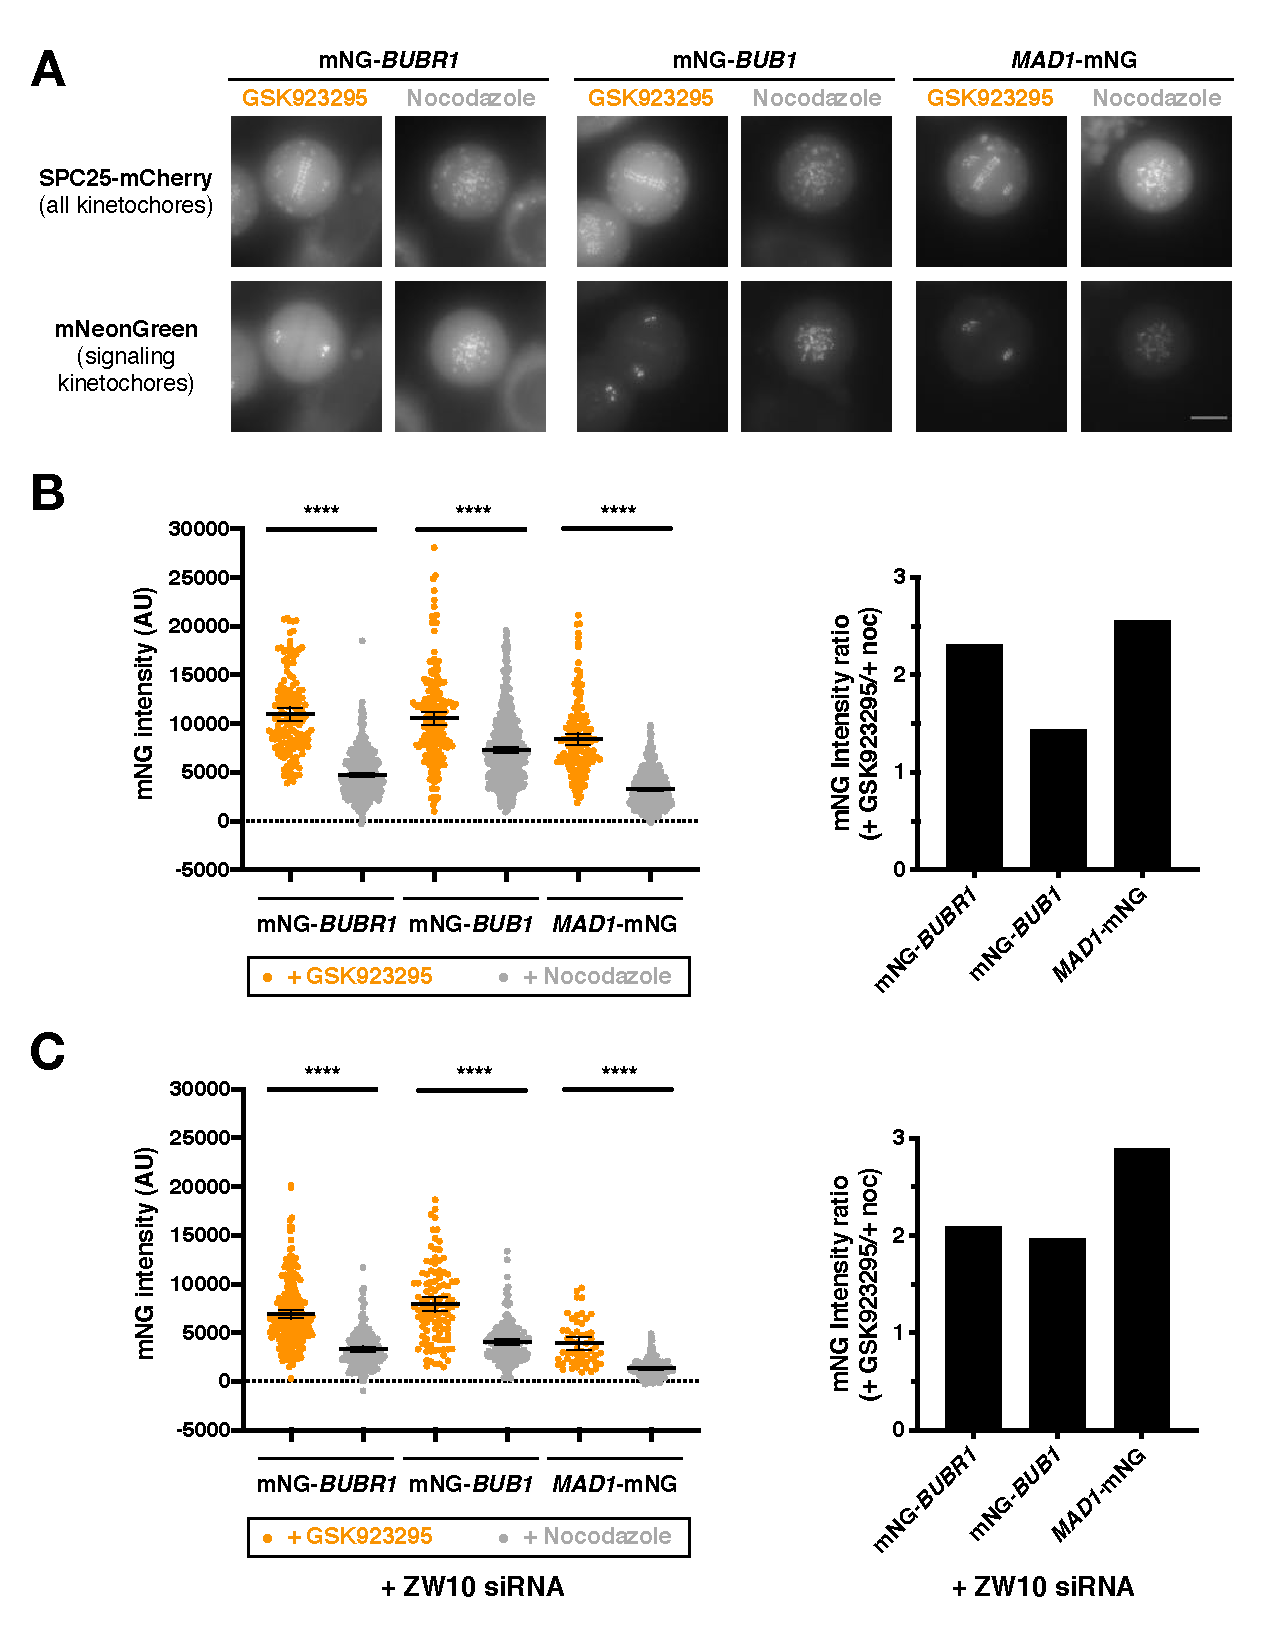
\includegraphics[width=\textwidth]{chapters/figures/SACProteinKinetochoreRecruitment.pdf}
    \phantomsubfiglabel{SACProteinKinetochoreRecruitment_Images} % subfigure A
    \phantomsubfiglabel{SACProteinKinetochoreRecruitment_Quantification} % subfigure B
    \phantomsubfiglabel{siZW10SACProteinKinetochoreRecruitment_Quantification} % subfigure C
    \caption{\textbf{\protein{BubR1} is more influential to SAC signaling strength and enriched at the few signaling kinetochores in GSK923295-treated cells than \gene{Bub1} and \protein{Mad1}.}}
    \noindent\justifying Lauren Humphrey-Stark performed all imaging experiments and data analysis involved in this figure. \myref{SACProteinKinetochoreRecruitment_Quantification,siZW10SACProteinKinetochoreRecruitment_Quantification} were reproduced from one of my first-author manuscripts in preparation. (A) Mitotic duration (NEBD to anaphase onset) of HeLa-A12 cells with \Latin{in situ} mNeonGreen-tagged \gene{BubR1}, \gene{Bub1}, or \gene{Mad1} in the presence of 330 nM nocodazole or 236 nM GSK923295. Cells were transfected with either an mNeonGreen-targeting siRNA to knock down the corresponding SAC gene (left panel) or a negative control siRNA (right panel). (B) Exemplary micrographs showing cells from the three HeLa-A12 cell lines treated with nocodazole or GSK923295. Spc25-mCherry labeled all kinetochores. Scale bar, \SI{10}{\micro m}. (B) Quantification of mNeonGreen signals at individual signaling kinetochores from experiments illustrated in (B). Each dot represents the measurement from one signaling kinetochore. Error bars represent 95\% confidence intervals of the mean. Results from at least two independent experiments are shown. Pairwise ratios between the average mNeonGreen signals at individual signaling kinetochores of GSK923295-treated cells and nocodazole-treated cells in (C).
    % Bub1/BubR1 recruitment data with knockdown of the RZZ complex compared with those with no siRNA deviate greatly from Zhang et al., 2019
\label{SACProteinKinetochoreRecruitment}
\end{figure}


\section{The chemical equilibrium between the activity of \protein{Mps1} and counteracting phosphatases at signaling kinetochore is the same in nocodazole- and GSK923295-treated HeLa-A12 cells}

The observed difference in the recruitment of SAC proteins on a per kinetochore basis in nocodazole- and GSK923295-treated cells may be alternatively attributed to a potential shift in the degree of phosphorylation of MELT motifs, according to a previous study \cite{MPS1senor}. To test this hypothesis in the HeLa-A12 cell line, we probed the equilibrium between the activity of kinases (mainly \protein{Mps1}) and counteracting phosphatases at the kinetochore (hereinafter referred to as \protein{Mps1}'s activity for simplicity) using a similar phosphorylation sensor (MPS1sen-KT) from this study. The only difference between our version of the MPS1sen-KT and the original design is that we used mNeonGreen/mScarlet-I as the acceptor/donor combination, which suits our confocal microscopy setup. The expression cassette of the recombinant sensor is under the regulation of TRE and stably integrated into the genome of HeLa-A12 cells via Cre-\bacterialgene{lox} RMCE. The acceptor and the donor has a fixed $1 : 1$ stoichiometry by design and the recombinant sensor was mostly intact in the cell (with no major partial degradation species like mScarlet-I-SPC24 alone; see \myref{MPS1sen-KT_Images}). Therefore, the ratio between the green channel readout and the raw FRET channel readout (even without corrections for the cross-excitation of the acceptor and the bleed-through of donor fluorescence) can be employed as a normalized measurement of the FRET efficiency (see \myref{FRETMetricTheory}) and therefore serve an indicator of \protein{Mps1}'s activity.

\begin{figure}
    \centering
    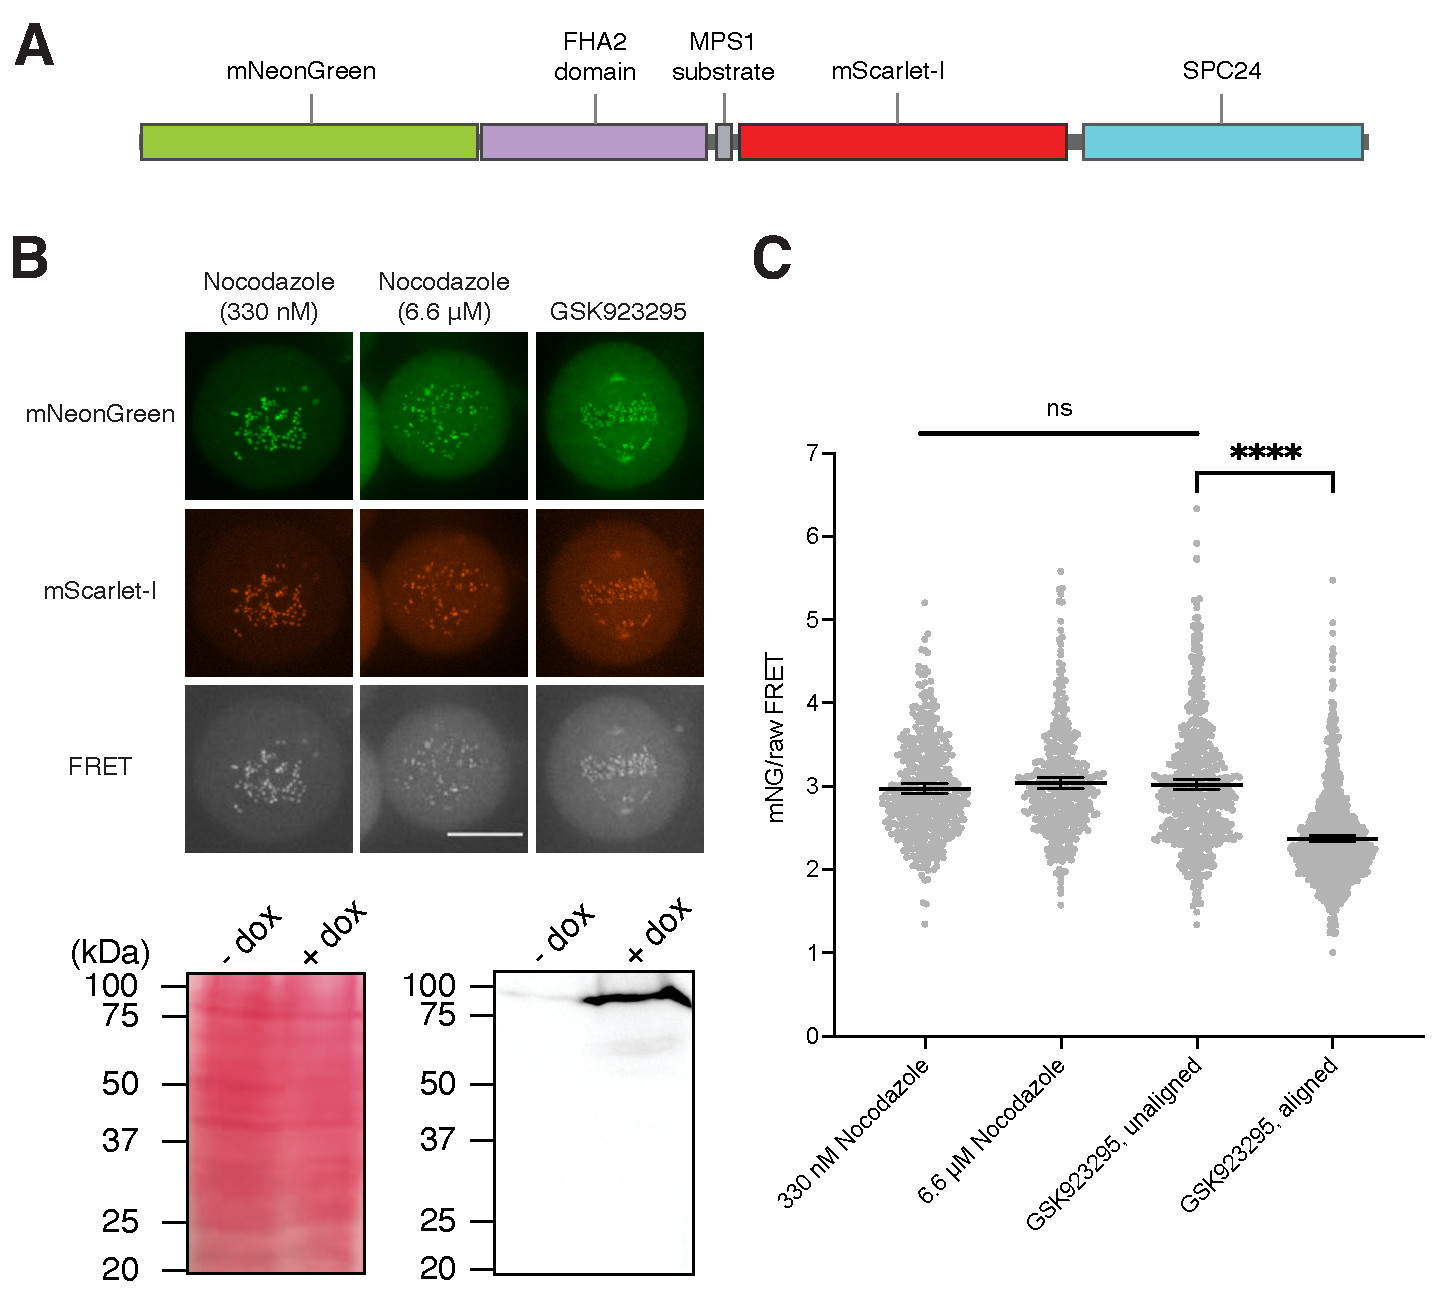
\includegraphics[width=0.95\textwidth]{chapters/figures/MPS1sen-KT.pdf}
    \phantomsubfiglabel{MPS1sen-KT_Scheme} % subfigure A
    \phantomsubfiglabel{MPS1sen-KT_Images} % subfigure B
    \phantomsubfiglabel{MPS1sen-KT_FRETMetric} % subfigure C
    \caption{\textbf{No difference in the \protein{Mps1}-phosphatases equilibrium at signaling kinetochores was detected in HeLa A12 when cells were treated with different drugs at various concentrations.}}
    \noindent\justifying (A) The design scheme of MPS1sen-KT. The \protein{Mps1} substrate sequence is \Peptide{LLEDGTLAINW}.
    % explain how it works
    The only difference between our sensor and the original design \cite{MPS1senor} is that we replaced the donor/acceptor pair with mNeonGreen/mScarlet-I, which works better with our imaging setup. (B) Top panel: representative images of cells expressing MPS1sen-KT. MPS1sen-KT was recruited to both unaligned signaling kinetochores (in Nocodazole- and GSK923295-treated cells) and aligned non-signaling kinetochores (in GSK923295-treated cells) via its C-terminal \protein{Spc24} module. Brightness and contrast have been adjusted but the look-up table for each channel (row) is universal for different groups (column). Scale bar, \SI{10}{\micro m}. Bottom panel: using an antibody against DsRed2 (which can detect many RFPs including mScarlet-I), we confirmed that MPS1sen-KT (with a theoretical molecular weight of \SI{97.2}{kDa}) can be induced by doxycycline to express as a full-length protein with negligible partial degradation or cleavage products in the RMCE HeLa-A12 cells (right blot). A Ponceau S staining of the same blot before membrane blocking (left blot) serves as the loading control. (C) A summary of a normalized FRET metric (mNeonGreen signal/FRET signal) in HeLa A12 cells treated with different drugs at various concentrations. Each gray dot represents a single kinetochore measurement. Data were compiled from at least two independent experiments (more than 40 cells in total for each group). Mean values $\pm 95\%$ confidence intervals are overlaid. Data from cells treated with \SI{45}{nM}, \SI{90}{nM}, and \SI{200}{nM} GSK923295 were pooled together (they have no significant difference from one another) to simplify the presentation. The Welch's ANOVA test [$W(\text{DF}n, \text{DF}d) = 1.339 (2.000, 917.0)$, $P = 0.2626$] was performed for the first 3 columns (signaling kinetochores). The unpaired $t$-test with Welch's correction ($P < 0.0001$) was performed to compare aligned non-signaling kinetochores with unaligned signaling kinetochores in GSK923295-treated cells. Statistical tests were done in Prism 9.
    \label{MPS1sen-KT}
\end{figure}

We confirmed that MPS1sen-KT recruited to unaligned kinetochores in both nocodazole- and GSK923295-treated cells had lower FRET efficiencies (higher activities of \protein{Mps1}) compared to MPS1sen-KT recruited to kinetochores aligned at metaphase plates in GSK923295-treated cells, consistent with the previous study \cite{MPS1senor}. However, in contrast to \cite{MPS1senor}, we did not observe any difference in \protein{Mps1}'s activity at unaligned kinetochores in nocodazole- versus GSK923295-treated cells. This was irrelevant to the concentrations of respective drugs and the reason for the conflicting observations may be explained by cell line-specific effects. As far as the HeLa-A12 cell line is concerned, the difference in the numbers of SAC proteins recruited per signaling kinetochore in nocodazole- and GSK923295-treated cells should be mainly attributed to the difference in the total number of signaling kinetochores in the cell, which all compete for the limited pool of SAC protein based on the law of mass action.

% It has been reported previously that the average localization levels of endogenously tagged HA-mCherry-\protein{Bub1} to signaling kinetochores in a CRISPR-Cas9-edited HeLa cell line treated with either \SI{250}{nM} of GSK923295 or \SI{6.6}{\micro M} of nocodazole were not significantly different \cite{MPS1senor}. One possible explanation is that the much higher concentration of nocodazole in the aforementioned study may contribute to a more complete breakdown of spindles and a higher number of phosphorylated MELT motifs, while the higher concentration of GSK923295 and the lack of filtering of cells based on the total number of unaligned chromosomes could mean more signaling kinetochores in GSK923295-treated cells.

%This observation contrasts with the previous report that the average localization levels of endogenously tagged HA-mCherry-Bub1 to signaling kinetochores in a CRISPR-Cas9-edited HeLa cell line treated with either 250 nM of GSK923295 or 6.6 μM of nocodazole were not significantly different (Kuijt et al., 2020). One possible explanation is that the much higher concentration of nocodazole in the aforementioned study may contribute to a more complete breakdown of spindles and a higher degree of phosphorylation of MELT motifs, while the lack of filtering of GSK923295-treated cells based on the number of unaligned chromosomes would lead to similar average numbers of signaling kinetochores in the Nocodazole- and GSK923295-treated cells. We also cannot rule out the possibility that the differences reflect different Bub1 expression levels or kinase/phosphatase activities in the HeLa cell lines used.